
\documentclass[12pt]{article}
\usepackage[a4paper, margin=.30in]{geometry}
\usepackage{graphicx ,
            wrapfig,
            xcolor, 
            enumerate,
            amsmath,
			fontenc,
			tcolorbox,circuitikz,tikz,bm
            }
			\usepackage{pgfplots}
\pgfplotsset{compat=newest}
\usepgfplotslibrary{fillbetween}
%\usepackage{scalerel}
%\usepackage{pict2e}
%\usepackage{tkz-euclide}
%\usetikzlibrary{calc}
%\usetikzlibrary{patterns,arrows.meta}
%\usetikzlibrary{shadows}
%\usetikzlibrary{external}

%%pgfplots
\usepackage{pgfplots}
%\pgfplotsset{compat=newest}
%\usepgfplotslibrary{statistics}
%\usepgfplotslibrary{fillbetween}

\newcommand\headerMe[2]{\noindent{}#1\hfill#2}
\renewcommand{\thesection}{\Roman{section}}

\author{Zakaria HAOUZAN}
\date{\today}

\begin{document}
% headers --------------
\headerMe{Matière : Physique-Chimie}{Professeur : Zakaria HAOUZAN}\\
\headerMe{Unité : Mécanique }{Établissement : Lycée SKHOR qualifiant}\\
\headerMe{Niveau : 2BAC-SM-PC}{Heure : 2H}\\

% ------Content ________
\begin{center}

    \Large{Leçon $N^{\circ} 13 $: \color{red}Mouvement des satellites et des planètes}
\end{center}

%\begin{wrapfigure}[10]{r}{0.5\textwidth}
%    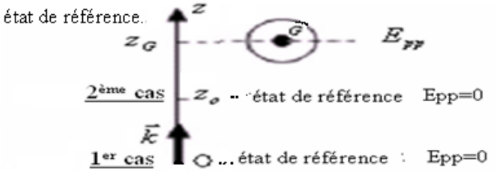
\includegraphics[width=0.5\textwidth]{./img/img00.png}
%\end{wrapfigure}

\section{Rappel de quelques propriétés des ellipses : }
\begin{wrapfigure}{r}{0.3\textwidth}
	\vspace{-2cm}
	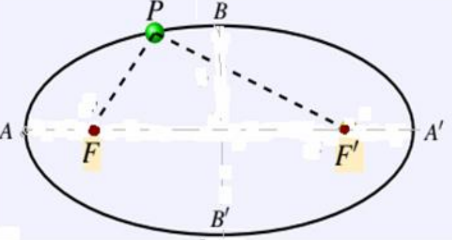
\includegraphics[width=0.3\textwidth]{./img_00.png}
\end{wrapfigure}


On rappel quelques propriétés de l'ellipse : F et F' sont les foyers de l'ellipse .

[A, A'] : est le grand axe de l'ellipse il mesure 2a. (a:c'est la longeur demi-grande axe).

[B,B'] : est le petit axe de l'ellipse il mesure 2b, (b:c'est la longeur du demi-petit axe)

Tout point P de l'ellipse vérifie la relation  suivante : PF + PF' = 2a = Cste


\section{Les lois de Kepler.}

\section*{La 1 ère loi de Kepler:}
\begin{wrapfigure}{r}{0.3\textwidth}
	\vspace{-2cm}
	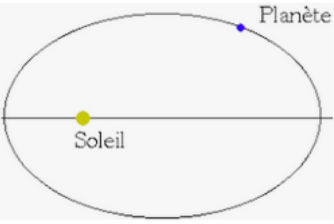
\includegraphics[width=0.3\textwidth]{./img_01.png}
\end{wrapfigure}
Dans le système solaire la trajectoire de chaque planète est une ellipse dont le soleil occupe l'un de ses foyers.



\section*{La 2 ème loi de Kepler:}
\begin{wrapfigure}{r}{0.3\textwidth}
	\vspace{-2cm}
	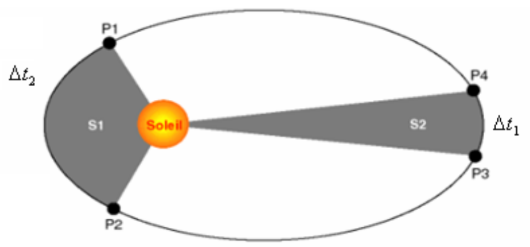
\includegraphics[width=0.3\textwidth]{./img_03.png}
\end{wrapfigure}
Cette loi est aussi appelée "loi des aires".Le rayon vecteur qui joint une planète au soleil balaie des surfaces égales dans des temps égaux

Le segment [Soleil, Planète] balaie la même surface pendant le même temps.
$s_1 = s_2$ et $\Delta{t_1} = \Delta{t_2}$

La vitesse de rotation dela planète autour du soleil varie selon son éloignement d'elle.
Lorsque la planète se rapproche du soleil sa vitesse augmente et au fur et à mesure qu'elle s'éloigne du soleil sa
vitesse diminue de telle façon que la surface balayée pendant le même temps est la même.


\section*{La 3 loi de Kepler:}
Les carrés des temps de révoltions sont proportionnels aux cubes des grands axes des orbites. On en déduit le rapport suivant :$$\frac{T^2}{a^3} = K$$

T :est la période de révolution .

a: le demi-grand axe.

K : est une constante qui s'exprime en $(s^2/m^3)$ dans le système international d'unités.

En conséquence les planètes lointaines du soleil sont les plus lentes.
\begin{tcolorbox}
Remarque : La 3
ème loi de Kepler pour les planètes dont les orbites sont circulaires de rayon est : $\frac{T^2}{r^3} = K$

\end{tcolorbox}

\section{Etude du mouvement d’une planète autour du soleil: }

\subsection{La gravitation universelle: }
\begin{wrapfigure}{r}{0.3\textwidth}
	\vspace{-2cm}
	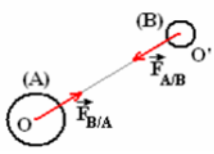
\includegraphics[width=0.3\textwidth]{./img_04.png}
\end{wrapfigure}
La gravitation universelle est un phénomène selon lequel tous les corps matériels s'attirent réciproquement de façon
proportionnelle à leur masse et inversement proportionnelle au carré de la distance qui les sépare.

Entre deux corps matériels A et B séparés d'une distance (d) s'exerce une action mutuelle attractive dont les forces $\vec{F_{A/B}}$ et $\vec{F_{B/A}}$ ont : 

\begin{itemize}

	\item même droite d'action.
	\item même intensité.
	\item des sens opposés:
	\item l'intensité commune des deux forces : $F=F_{A/B} = F_{B/A} = G.\frac{m_A.m_B}{d^2}$
\end{itemize}

$F_{A/B}$ : l'intensité de la force exercée par le corps A sur le corps B (en N)

$F_{B/A}$ : l'intensité de la force exercée par le corps B sur le corps A (en N)

$m_A$ : masse du corps A (en Kg)

$m_B$ : masse du corps B (en Kg)

$d$ : distance entre le corps A et le corps B (en m)

$G = 6,67.10^{-11} $ la constante de gravitation universelle $(N.m^2/Kg)$

\begin{tcolorbox}
Cette loi se généralise sur les corps terrestres sphériques à répartition massiques régulière comme la terre et la lune , dans ce cas la distance (d) est la distance entre leurs centres.
\end{tcolorbox}

\subsection{Etude du mouvement de révolution de la planète aurtour du soleil:}
\begin{wrapfigure}{r}{0.3\textwidth}
	\vspace{-2cm}
	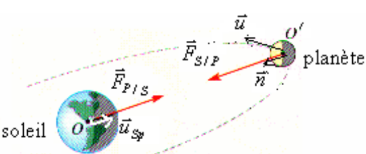
\includegraphics[width=0.3\textwidth]{./img_05.png}
\end{wrapfigure}

On considère une planète de masse $m_p$ dans un mouvement circulaire autour du soleil de masse $m_s$.
\\-Le système étudié {la planète}
\\-Bilan des forces: la planète dans son mouvement autour du soleil est soumise à la seul force d'attraction universelle
exercée sur lui par le soleil.
$$\vec{F_{S/P}} = -G.\frac{m_s.m_p}{r^2}.\vec{u_{sp}}$$ r: rayon de l'orbite de la planète

-Application de la deuxième loi de Newton: 

\begin{itemize}
	\item $\sum{\vec{\vec{F_{ext}}}} \Rightarrow \vec{F}=m.\vec{a_G}$ 
	\item $\vec{a_G} = -G.\frac{m_S}{r^2}.\vec{u_{sp}}$
	\item Donc le vecteur accélération $\vec{a_G}$ a le même sens que $\vec{F_{s/p}}$ qui est centripète.
	\item Par conséquence l'accélération tangentielle est nulle : $a_t = \frac{dv}{dt} = 0$ alors v=cst
	\item Par projection de la relation (1) sur la normale dans le repère de Frenet $(O', \vec{u},\vec{n})$ : $F_{s/p} = m_p.a_G$ $$G.\frac{m_s.m_p}{r^2} = m_p.\frac{v^2}{r}$$ donc $v = \sqrt{G.\frac{m_s}{r}}$
\end{itemize}

La vitesse de la planète est constante et son rayon est constant, donc son mouvement est circulaire uniforme.

\section*{Expression de la période de révolution : }

Le mouvement de la planète est circulaire uniforme, sa période : $T=\frac{2.\pi}{\omega}$ $\omega = \frac{v}{r}$ avec $v = \sqrt{G.\frac{m_s}{r}}$ 

donc  $T = 2.\pi.\sqrt{\frac{r^3}{G.m_s}}$

Donc on a : $T^2 = 4.\pi^2.\frac{r^3}{G.m_s}$ $\Rightarrow$ $\frac{T^2}{r^3} = \frac{4.\pi^2}{G.m_s}$

\subsection{Cas d'un satellite artificiel :}
\begin{wrapfigure}{r}{0.3\textwidth}
	\vspace{-2cm}
	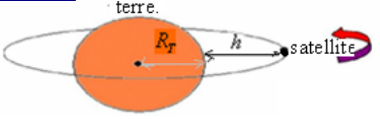
\includegraphics[width=0.3\textwidth]{./img_06.png}
\end{wrapfigure}
Le satellite est en rotation autour de la terre. 

Si le satellite se trouve à une altitude h de la surface de la terre , la force de gravitation universelle qui s'applique sur lui par la terre a pour intensité $F_{T/S} = G.\frac{M_T.m_s}{(R_T + h)^2}$

En appliquant la deuxième loi de Newton sur le satellite on a : $\vec{F_{T/S}} = m_s.\vec{a_G}$ Par projection sur la normale on a : $F_{T/S} = m_s.a_N$
donc $$G.\frac{M_T.m_s}{(R_T + h)^2} = m_s.\frac{v^2}{R_T + h}$$

car la force de gravitation est centripète donc $v = \sqrt{\frac{M_T}{R_T + h}}$


Et la période de révolution du satellite est $T = \frac{2.\pi}{\omega}$ et $\omega = \frac{v}{r}$ avec $v = \sqrt{\frac{M_T}{R_T + h}}$

donc $T=w.\pi.\sqrt{\frac{(R_T)}{G.M_T}}$

\begin{tcolorbox}
Le satellite géostationnaire apparait immobile par rapport à un point de la surface de la terre si sa période de
révolution Test égale à la période de révolution de la terre autour d'elle-même donc T=24h. et ceci se réalise lorsque le satellite
se trouve à l'altitude h=3600km.
\end{tcolorbox}

%wfg---------------------------------------------------------------sf 


%\begin{center}
   %\begin{tabular}{ |c|c|c|c|c|c|c| }
      %\hline
      %km & hm & dam & \bf{m} & dm & cm & mm \\
      %\hline
        %&   &    &  &   &   & \\
%\hline
%\end{tabular}
%On place un seul nombre dans chaque case.
%\end{center}
%\begin{center}
   %\begin{tabular}{ |c|c|c|c|c|c|c| }
      %\hline
      %$km^2$ & $hm^2$ & $dam^2$ & \bf{$m^2$} & $dm^2$ & $cm^2$ & $mm^2$ \\
      %\hline
        %&   &    &  &   &   & \\
%\hline
%\end{tabular}
%\end{center}


\end{document}

